%
% Requisitos levantados para o projeto de alertas de medicação
% via dispositivo móvel.
%
% por,
% Bruno Romero de Azevedo,
% Hugo Stefan Kaus Puhlmann,
% Thiago
% Grupo de Sistemas de Computação Móvel - GMob
% ------------------------------------------------------------------%

\documentclass[12pt,a4paper]{article}

\usepackage[brazilian]{babel}
\usepackage[utf8]{inputenc}

\usepackage[T1]{fontenc}
\usepackage{ae,aecompl}

\usepackage{graphicx}

\begin{document}
\title{Requisitos para aplicação de alertas de medicação via dispositivo móvel}
\author{Bruno Romero de Azevedo \\
		\texttt{brunodea@inf.ufsm.br} \and
		Hugo Stefan Kaus Puhlmann \\
		\texttt{puhlmann@inf.ufsm.br} \and
		Thiago Lopes Trugillo da Silveira \\
		\texttt{thiago@inf.ufsm.br}}
\date{\today}
\maketitle

\section{Elementos Básicos}

	\subsection{De ordem geral}
		\begin{itemize}
			\item Múltiplos perfis para permitir o uso da aplicação entre vários pacientes utilizando apenas um
				  dispositivo móvel.
			\item Os medicamentos devem ser únicos. (Vários perfis podem compartilhar um mesmo medicamento)
			\item Possibilidade de expansão para o uso de servidor remoto.
			
				  Sendo utilizado para:
				  \begin{itemize}
				  	\item Ajuste das informações em um site.
				  	\item Sincronização dessas informações com o aplicativo em qualquer celular.
				  	\item Inclusive poderia ser ajustado para apenas o médico ser capaz de alterar os dados.
				  \end{itemize}
		\end{itemize}
		
	\subsection{Com relação aos Medicamentos}
		\begin{itemize}
			\item Nome do medicamento.
			\item Para cada dosagem do medicamento, considera-o como um medicamento diferente.
				  
				  Exemplo: \emph{Diasepam 500mg} e \emph{Diasepam 200mg} vão ser tratados como dois medicamentos 
				  				  diferentes.
		\end{itemize}
		
	\subsection{Com relação aos Perfis}
		\begin{itemize}
			\item Cada perfil tem uma lista com os medicamentos que lhe interessam.
			\item Relacionado com cada medicamento da lista de medicamentos pode-se:
				\begin{enumerate}
					\item Adicionar notas sobre ele.
					\item Ajustar as horas (hora e data de início) em que o alarme é acionado para ele.
					
						As horas podem ser:
						\begin{enumerate}
							\item \emph{Fixas:} O usuário digita exatamente os horários em que é para tocar o 
											    alarme.
							\item \emph{Periódicas:} O usuário simplesmente escolhe a data inicial e a 
													 periodicidade em que é para usar o medicamento.
													 Por exemplo, de 2 em 2 horas.
						\end{enumerate}
				\end{enumerate}
		\end{itemize}
		
	\subsection{Com relação ao Alarme}
		\begin{itemize}
			\item Na tela de medicamentos que ativaram o alarme, deve-se indicar qual sua procedência. Ou seja,
				  a que perfil pertence.
			\item O alarme deve mostrar de alguma forma (seja abrindo o aplicativo ou na própria mensagem que
				  aparece junto ao alarme) as notas relacionadas ao medicamento em questão.
		\end{itemize}
		
\section{Telas de Exemplo}
	\begin{figure}[htb]
		\begin{center}
			\leavevmode
			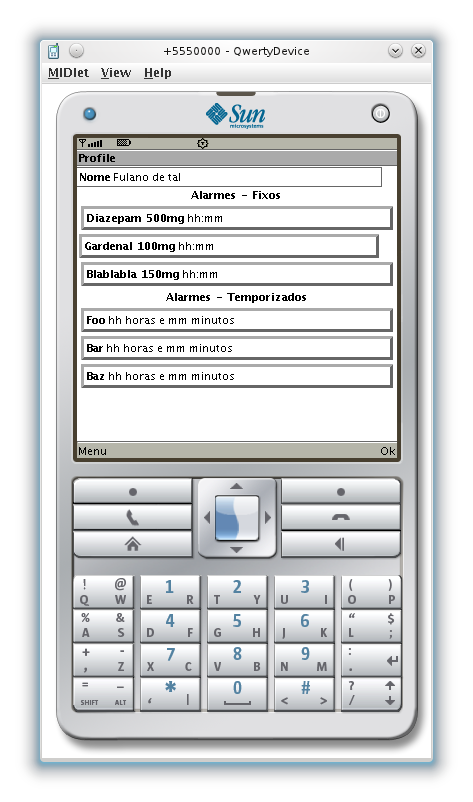
\includegraphics[scale=1]{medalert-profile.png}
		\end{center}
		\caption{Tela básica (geral) com os componentes de um perfil do usuário.}
		\label{fig:medalert-profile}
	\end{figure}
	
	\begin{figure}[htb]
		\begin{center}
			\leavevmode
			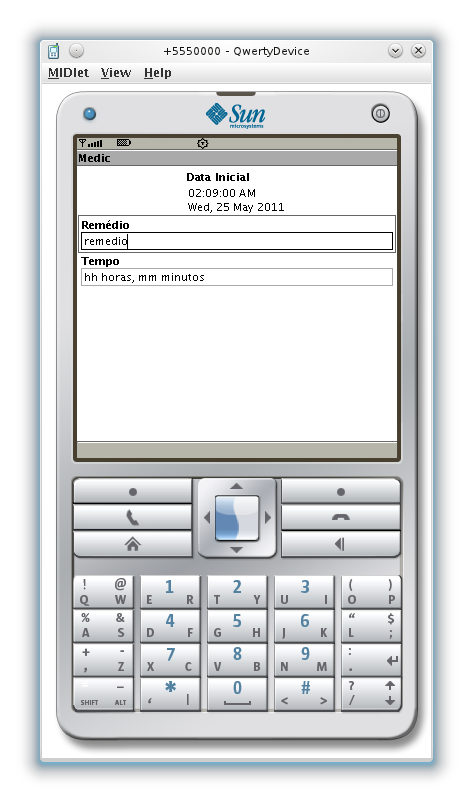
\includegraphics[scale=1]{medalert-medic-temporizado.png}
		\end{center}
		\caption{Tela onde se setam os horários em que determinada medicação vai disparar um alarme.}
		\label{fig:medalert-medic-temporizado}
	\end{figure}

\end{document}
